\subsection{Solar Input Module (SI) }
\label{sec:SI}

The Solar Input Module (SI) filters and scales the output voltage of the solar panels.
Given the physical distance between panel and SI of approx. \SI{20}{\meter}, the inputs are susceptible
to overvoltage due to atmospheric disturbances. The solar panel output voltage should also be
digitized by \mu M.


\subsubsection{Requirements}

The voltage applied to the analog input of \mu M must not exceed \SI{3.3}{\volt}.


\subsubsection{Implementation}


\begin{figure}[h]
    \centering
    \includegraphics[width=0.5\textwidth]{PO/SI/SI}
    \caption{SI - schematic, n = 1,2}
\end{figure}

\begin{table}[H]
    \centering
    \begin{threeparttable}[b]
        \begin{tabularx}{\linewidth}{ >
                    {\hsize=.25\hsize}X >
                    {\hsize=0.5\hsize}X >
                    {\hsize=.25\hsize}X  >
                    {\hsize=.5\hsize}X >
                    {\hsize=.25\hsize}X  >
                    {\hsize=3\hsize}X
            }
                  & \multicolumn{4}{c}{pin} &                                                    \\
            \cmidrule(lr){3-6}
            Id    & Net                     & Nb. & Name       & Type                 & Function \\
            \midrule
            $D_1$ & .S\textsubscript{n'c}   & 1   & \texttt{1} & \Gnd                 &          \\
            $D_1$ & \Gnd                    & 2   & \texttt{2} & \Gnd                 &          \\
            $D_2$ & .S\textsubscript{n}     & 1   & \texttt{1} & \Gnd                 &          \\
            $D_2$ & \Gnd                    & 2   & \texttt{2} & \Gnd                 &          \\
            $D_3$ & .S\textsubscript{n}     & 1   & \texttt{A} &                      &          \\
            $D_3$ & .S\textsubscript{n'}    & 2   & \texttt{C} &                      &          \\
            $R_1$ & .S\textsubscript{n}     & 1   & \texttt{1} & \leftarrow           &          \\
            $R_1$ & .S\textsubscript{n'c}   & 2   & \texttt{2} & \leftrightsquigarrow &          \\
            $R_2$ & .S\textsubscript{n'c}   & 1   & \texttt{1} & \rightarrow          &          \\
            $R_2$ & \Gnd                    & 2   & \texttt{2} &                      &          \\
        \end{tabularx}
    \end{threeparttable}
    %\caption{WD - Pin mapping}
\end{table}

\begin{table}[H]
    \centering
    \begin{threeparttable}[b]
        \begin{tabularx}{\linewidth}{
                >{\hsize=0.25\hsize}X
                >{\hsize=0.75\hsize}X
                >{\hsize=1.25\hsize}X
                >{\hsize=0.75\hsize}X
                >{\hsize=2\hsize}X}
            \toprule
            Id    & Desc                                & Order Code         & Package  & Rationale \\
            \midrule
            $D_1$ & \cite{noauthor_cdsod323-txxsc_2019} & CDSOD323-T03SC/820 & SOD-323  &           \\
            $D_2$ & \cite{noauthor_cdsod323-txxsc_2019} & CDSOD323-T36SC/945 & SOD-323  &           \\
            $D_3$ & \cite{noauthor_cdba340l-hf_2009}    & CDBA340L-G/618     & DO-214AC &           \\
            $R_1$ & \SI{180}{\kilo\ohm}                 & generic            & 0603     &           \\
            $R_2$ & \SI{20}{\kilo\ohm}                  & generic            & 0603     &           \\
            \bottomrule
        \end{tabularx}
    \end{threeparttable}
    % \caption{WD Module - BOM}
    \label{table:wd1}
\end{table}

\begin{table}[H]
    \centering
    \begin{threeparttable}[b]
        \begin{tabularx}{\linewidth}{ >{\hsize=.15\hsize}X >{\hsize=1.35\hsize}X >{\hsize=1.5\hsize}X }
            \toprule
            Id & Issue                                & Potential solutions \\
            \midrule
            1  & reverse current of $D_3$ is too high & make further tests  \\
            \bottomrule
        \end{tabularx}
    \end{threeparttable}
    \caption{SI - issues}
\end{table}